\chapter{Prediction of the world's temperature}
\label{chap:two}

This chapter outlines several regression models, namely \textit{Polynomial Regression}, \textit{Ridge Regression}, and \textit{Lasso Regression} that are utilized to forecast the Earth's temperature in the current century. Additionally, machine learning models will consider three different scenarios.
\begin{enumerate}
  \item \coo\ emission remains the same as in 2021
  \item \coo\ emission drops yearly by 2\%
  \item \coo\ emission increases yearly by 2\%
\end{enumerate}
Figure ~\ref{fig:cumulative-co2-temperature} demonstrates correlation between normalized\footnote{Normalization is a common technique used for machine learning models. It helps avoid numerical issues during trainning phase and improves stability of some algorithms. } values of \coo\ emission and temperature anomalies.
It is noteworthy that all models used in the experiment use a \textit{cumulative} function of carbon dioxide emissions, whereby the total amount of emissions is accumulated, as opposed to measuring discrete values on a yearly basis. 
The \textit{cumulative} approach eliminates issues related to non-uniform \coo\ emissions on an annual basis, and furthermore incorporates a historical perspective on emissions.
It is worth to mention that models used for temperature predictions do not take into account absorbtion of \coo\ by forests that provide \textit{carbon sink}. It is estimated that forests can absorb 7.6 billion metric tonnes of \coo\ per year\cite{forest-absorbs} which unfortunately is only 3.5\% of 2021's \coo\ emission.
On the other hand, recent findings\cite{forest-emits}, discovered that Amazon rainforets emits now more \coo\ that it can absorbe and it has become a source of \coo\, rather than a sink. It appears that there is a need for further research and improved data quality and understanding in the field of climate change. 

\begin{figure}[H]
  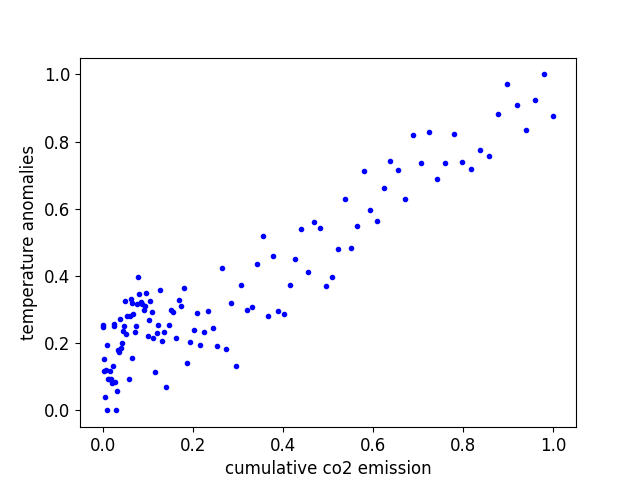
\includegraphics[width=\linewidth]{img/cumulative-co2-temperature.png}
  \caption{Corelation between normalized values of carbon dioxide emission and temperature anomalies}
  \label{fig:cumulative-co2-temperature}
\end{figure}

\clearpage
\section{Linear Regresion}
Result of \textit{Linear Regression} method are demonstrated on figure ~\ref{fig:linear-regression}. Line that approxymates the model is described by formula:
\[ y = 0.14551849x + 0.7704561  \]
Despite achieving a high coefficient of determination score of 0.86, the \textit{Linear Regression} model will not be utilized for predicting the Earth's temperature.
The following section of the chapter explores more advanced regression methods.
\begin{figure}[h]
  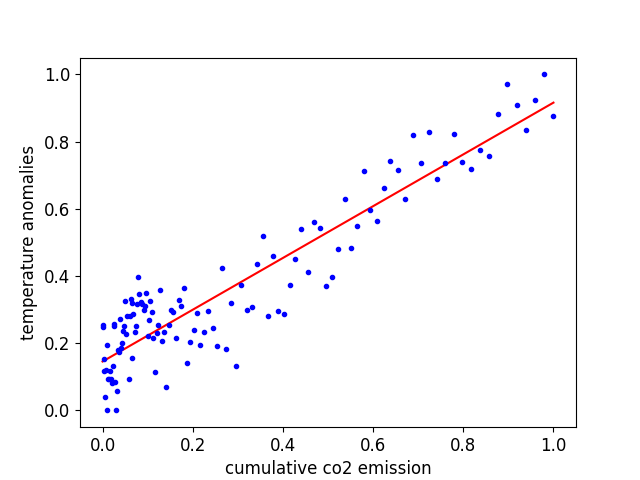
\includegraphics[width=\linewidth]{img/linear-regression.png}
  \caption{\textit{Linear Regression} model used for temperature anomalies prediction }
  \label{fig:linear-regression}
\end{figure}

\clearpage
\section{Polynomial Regression}
Result of \textit{Polynomial Regression} method used for anomalies prefiction are demonstrated on figure ~\ref{fig:polynomial-regression}. 
The dataset was partitioned into training and testing subsets using an 80/20 ratio. Coefficient of determination score equals 0.87 and it is sligtly higher than \textit{Linear Regression}
\begin{figure}[h]
  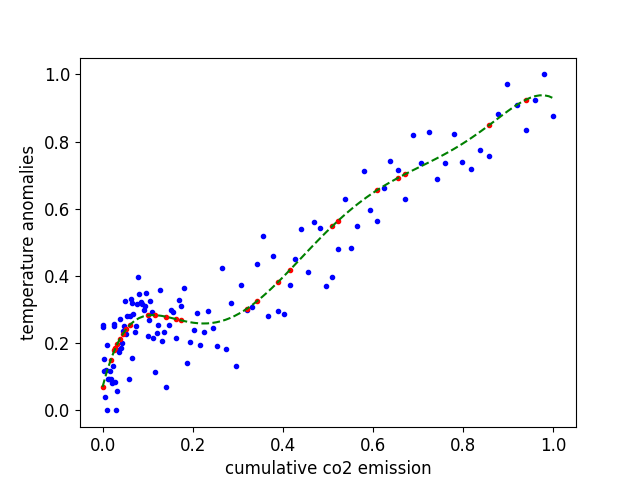
\includegraphics[width=\linewidth]{img/polynomial-regression.png}
  \caption{\textit{Polynomial Regression} model used for temperature anomalies prediction}
  \label{fig:polynomial-regression}
\end{figure}

Interesting results are visible on figure ~\ref{fig:polynomial-regression-result}, where three different scenarios were take into account. In all the cases the increase of temperature is, unfortunately, inevitable. 
Table ~\ref{tab:polynomial-regression-table} displays a representation of specific data points alongside the Earth's temperature.
\begin{table}[h]
\begin{tabular}{ |p{4cm}||p{2cm}|p{2cm}|p{2cm}|  }
 \hline
 & \textbf{2050} & \textbf{2075} & \textbf{2100} \\
 \hline
constant emission &  +2.16\degree C	& +3.11\degree C 	& +4.23\degree C \\
  drops yearly by 2\% &  +1.91\degree C &	+2.28\degree C &	+2.5\degree C  \\
  increases yearly by 2\% &  +2.54\degree C &	+5.17\degree C &	+11.37\degree C  \\
 \hline
\end{tabular}
\caption{Prediction of the the Earth's temperature in 2050, 2075 and 2100 using \textit{Polynomial Regression} model with different carbon dioxide emissions} 
\label{tab:polynomial-regression-table}
\end{table}
\begin{figure}[H]
  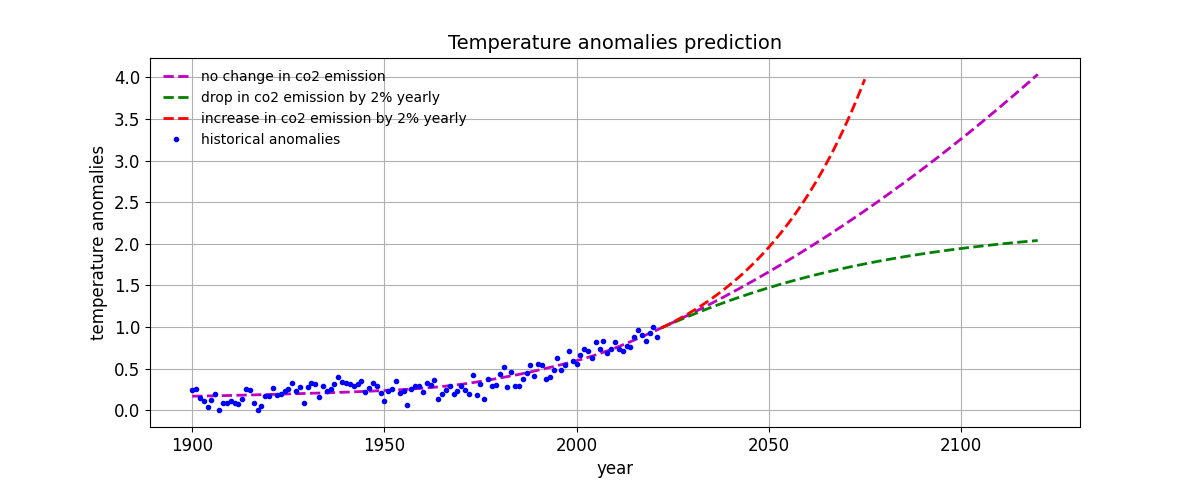
\includegraphics[width=\linewidth]{img/polynomial-regression-result.png}
  \caption{Polynomial Regression model used for temperature anomalies prediction}
  \label{fig:polynomial-regression-result}
\end{figure}
It is worth to mention that the results depicted on the figure ~\ref{fig:polynomial-regression-result} are derived from the chart ~\ref{fig:polynomial-regression}. Any data beyond 2021 represents a prediction generated by the primary model.

\clearpage
\section{Ridge Regression}
Result of \textit{Ridge Regression} method used for anomalies prefiction are demonstrated on figure ~\ref{fig:ridge-regression}. 
Similarly as for previous model, the dataset was partitioned into training and testing subsets using an 80/20 ratio. Coefficient of determination score equals 0.87 and it is the same as \textit{Polynomial Regression}
\begin{figure}[h]
  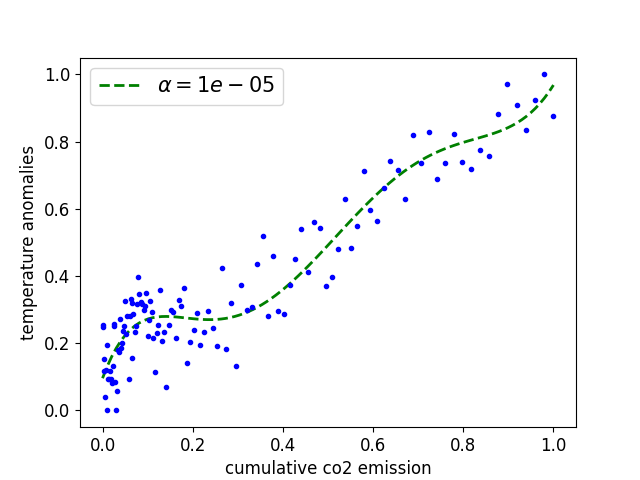
\includegraphics[width=\linewidth]{img/ridge-regression.png}
  \caption{Ridge Regression model used for temperature anomalies prediction}
  \label{fig:ridge-regression}
\end{figure}

\begin{table}[ht]
\begin{tabular}{ |p{4cm}||p{2cm}|p{2cm}|p{2cm}|  }
 \hline
 & \textbf{2050} & \textbf{2075} & \textbf{2100} \\
 \hline
constant emission &  +2.22\degree C	& +3.25\degree C 	& +4.46\degree C \\
  drops yearly by 2\% &  +1.96\degree C &	+2.36\degree C &	+2.61\degree C  \\
  increases yearly by 2\% &  +2.54\degree C &	+5.17\degree C &	+11.37\degree C  \\
 \hline
\end{tabular}
\caption{Prediction of the Earth's temperature in 2050, 2075 and 2100 using \textit{Ridge Regression} methods} 
\label{tab:ridge-regression-table}
\end{table}

\begin{figure}[H]
  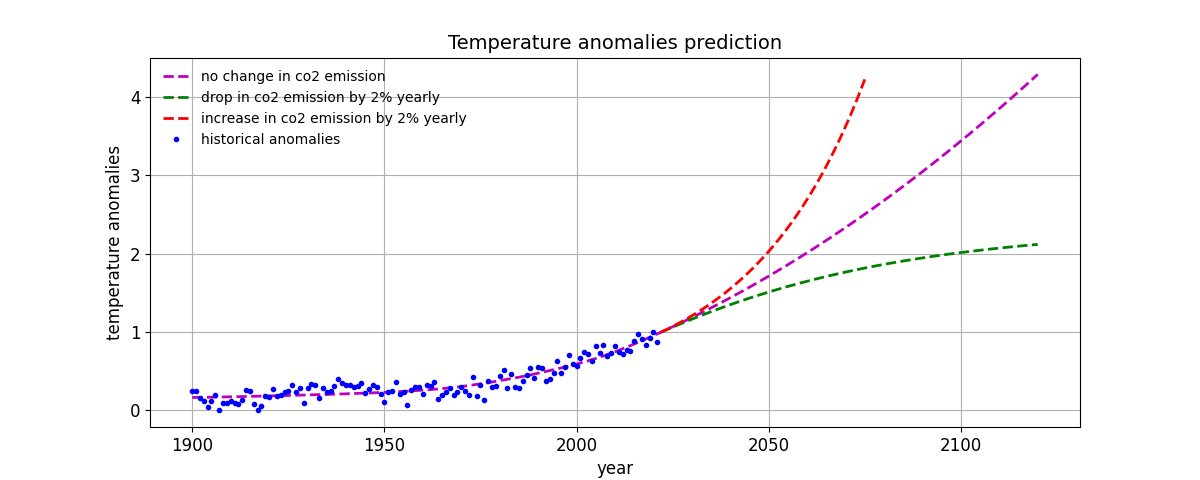
\includegraphics[width=\linewidth]{img/ridge-regression-result.png}
  \caption{Ridge Regression model used for temperature anomalies prediction}
  \label{fig:ridge-regression-result}
\end{figure}
It is worth to mention that the results depicted on the figure ~\ref{fig:ridge-regression-result} are derived from the chart ~\ref{fig:ridge-regression}. Any data beyond 2021 represents a prediction generated by the primary model.


\clearpage
\section{Lasso Regression}
Result of \textit{Lasso Regression} method used for anomalies prefiction are demonstrated on figure ~\ref{fig:lasso-regression}. 
Similarly as for previous model, the dataset was partitioned into training and testing subsets using an 80/20 ratio. Coefficient of determination score equals 0.87 and it is the same as \textit{Polynomial Regression}
\begin{figure}[h]
  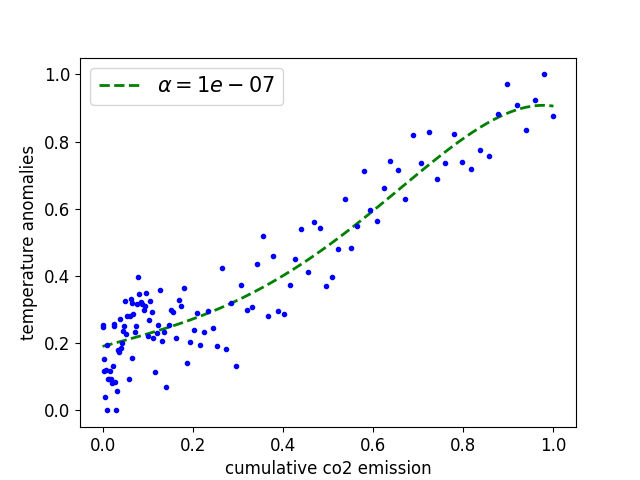
\includegraphics[width=\linewidth]{img/lasso-regression.png}
  \caption{Lasso Regression model used for temperature anomalies prediction}
  \label{fig:lasso-regression}
\end{figure}

\begin{table}[ht]
\begin{tabular}{ |p{4cm}||p{2cm}|p{2cm}|p{2cm}|  }
 \hline
 & \textbf{2050} & \textbf{2075} & \textbf{2100} \\
 \hline
constant emission &  +2.23\degree C	& +3.25\degree C 	& +4.45\degree C \\
  drops yearly by 2\% &  +1.97\degree C &	+2.36\degree C &	+2.62\degree C  \\
  increases yearly by 2\% &  +2.64\degree C &	+5.46\degree C &	+12.18\degree C  \\
 \hline
\end{tabular}
\caption{Prediction of the Earth's temperature in 2050, 2075 and 2100 using \textit{Lasso Regression} methods} 
\label{tab:lasso-regression-table}
\end{table}

\begin{figure}[H]
  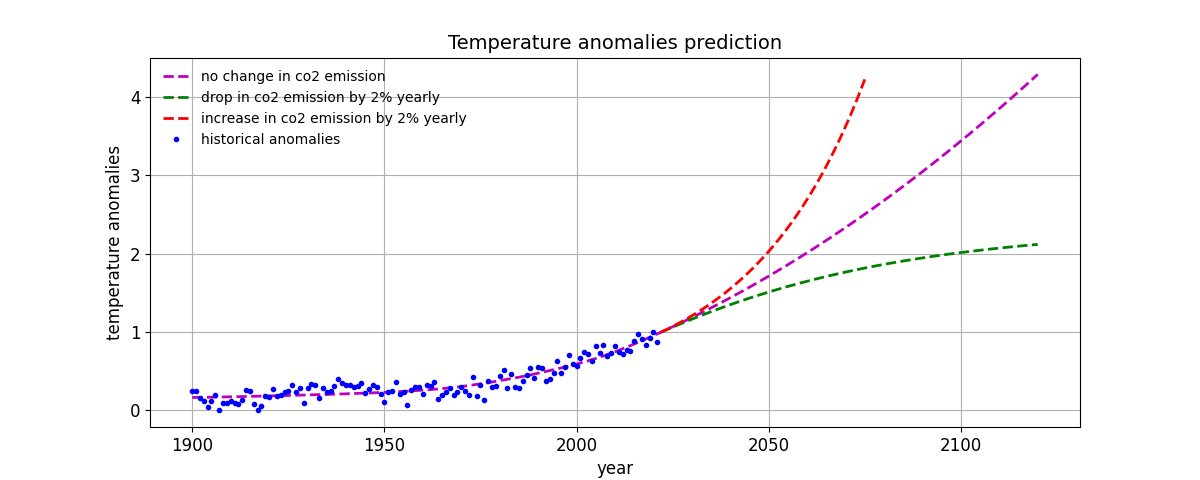
\includegraphics[width=\linewidth]{img/ridge-regression-result.png}
  \caption{\textit{Lasso Regression} model used for temperature anomalies prediction}
  \label{fig:lasso-regression-result}
\end{figure}
It is worth to mention that the results depicted on figure ~\ref{fig:lasso-regression-result} are derived from chart ~\ref{fig:lasso-regression}. Any data beyond 2021 represents a prediction generated by the primary model.

\section{Comparision of ML algorithms}
All models used for the Earth's prediction can be compared by \textit{coefficient of determination}\cite{coefficient}
\begin{table}[ht]
\begin{tabular}{ |p{5cm}||p{6cm}|  }
 \hline
 & \textbf{coefficient of determination score} \\
 \hline
Linear Regression &  0.86  \\
Polynomial Regression &  0.87  \\
Ridge Regression   &  0.87  \\
Lasso Regression   &  0.87  \\
 \hline
\end{tabular}
\caption{Comparision of coefficient of determination score for models used in the the Earth's temperature predictions} 
\label{tab:coefficient-table}
\end{table}
\textit{Polynomial, Ridge} and \textit{Lasso} regression got the same score. 
\\Additionally, based on tables ~\ref{tab:polynomial-regression-table}, ~\ref{tab:ridge-regression-table} and ~\ref{tab:lasso-regression-table}, predictions differ in a fraction of \degree C for historical data.
A similar experiment was conducted by Berkeley Earth, in which three scenarios were taken into account, SSP3-7.0 representing increasing, SSP1-2.6 decreasing, and SSP2-4.5 stabilizing \coo\ emissions.
\\Figure ~\ref{fig:poland-temperature-chart}, on the next page, shows results for Poland.
\\
\\SSP1-2.6 - represented by the green curve - with significantly lower greenhouse gas emissions, assumes net zero carbon dioxide worldwide by 2080. Under this scenario, overall average global warming is expected to reach approximately 1.8\degree C by 2100.
\\
\\SSP2-4.5 - represented by the orange curve - an intermediate emissions trajectory. This assumes that modern emissions levels stay approximately consistent through 2050, before gradually declining.  Under this scenario, net zero is not reached by 2100, and global average warming is expected to have reached approximately 2.7\degree C by 2100 and still be rising.  Among the scenarios, this is the closest to the world’s current behavior on emissions
\\
\\SSP3-7.0 - represented by the brown curve - a high emissions, high warming scenario, that assumes the world not only fails to curtail greenhouse gas emissions, but that emissions continue to rise. Under this scenario, carbon dioxide emissions are assumed to double by 2100; average global temperatures would reach approximately 3.6\degree C above pre-industrial baseline, more than doubling current levels of warming

\begin{figure}[ht]
  \includegraphics[width=\linewidth]{img/Poland-temperature-chart.png}
  \caption{Berkeley's Earth forecast for Poland}
  \label{fig:poland-temperature-chart}
\end{figure}

\begin{table}[H]
\begin{tabular}{ |p{5cm}||p{6cm}|  }
 \hline
 & \textbf{The Earth's temperature forecast} \\
 \hline
\rule{0pt}{3ex}  SSP1-2.6 & ~3.1\degree C  \\
\rule{0pt}{3ex}1. emission drops yearly by 2\% & 2.5\degree C - 2.62\degree C  \\
\hline
\rule{0pt}{3ex}  SSP2-4.5 & ~4\degree C  \\
\rule{0pt}{3ex}2. emission constant by 2\% & 4.23\degree C - 4.46\degree C  \\
 \hline
\end{tabular}
\caption{Comparision of Berkeley Earth's forecast and Regression's model forecast} 
\label{tab:compare-1}
\end{table}


\section{Summary}
Machine learning models have shown promise in predicting the Earth's temperature changes due to climate change.
However, there are still many challenges to be addressed, such as the selection of appropriate models and the resolution of data quality concerns. 
Nonetheless, these models serve as an invaluable resource for policymakers and scientists striving to gain deeper insights into and alleviate the repercussions of climate change.